%%%%%%%%%%%%%%%%%%%%%%%%%%%%%%%%%%%%%%%%%
% Beamer Presentation
% LaTeX Template
% Version 1.0 (10/11/12)
%
% This template has been downloaded from:
% http://www.LaTeXTemplates.com
%
% License:
% CC BY-NC-SA 3.0 (http://creativecommons.org/licenses/by-nc-sa/3.0/)
%
%%%%%%%%%%%%%%%%%%%%%%%%%%%%%%%%%%%%%%%%%

%----------------------------------------------------------------------------------------
%	PACKAGES AND THEMES
%----------------------------------------------------------------------------------------

%\documentclass[UTF8,aspectratio=169,14pt]{ctexbeamer}
\documentclass[UTF8,aspectratio=169]{ctexbeamer}
\usepackage{hyperref}
\hypersetup{
	colorlinks=true,
	linkcolor=red,
	anchorcolor=blue,
	citecolor=green
}

\mode<presentation> {
	
	% The Beamer class comes with a number of default slide themes
	% which change the colors and layouts of slides. Below this is a list
	% of all the themes, uncomment each in turn to see what they look like.
	
	%\usetheme{default}
	%\usetheme{AnnArbor}
	%\usetheme{Antibes}
	%\usetheme{Bergen}
	%\usetheme{Berkeley}
	%\usetheme{Berlin}
	%\usetheme{Boadilla}
	%\usetheme{CambridgeUS}
	%\usetheme{Copenhagen}
	%\usetheme{Darmstadt}
	%\usetheme{Dresden}
	%\usetheme{Frankfurt}
	%\usetheme{Goettingen}
	%\usetheme{Hannover}
	%\usetheme{Ilmenau}
	%\usetheme{JuanLesPins}
	%\usetheme{Luebeck}
	\usetheme{Madrid}
	%\usetheme{Malmoe}
	%\usetheme{Marburg}
	%\usetheme{Montpellier}
	%\usetheme{PaloAlto}
	%\usetheme{Pittsburgh}
	%\usetheme{Rochester}
	%\usetheme{Singapore}
	%\usetheme{Szeged}
	%\usetheme{Warsaw}
	
	% As well as themes, the Beamer class has a number of color themes
	% for any slide theme. Uncomment each of these in turn to see how it
	% changes the colors of your current slide theme.
	
	%\usecolortheme{albatross}
	%\usecolortheme{beaver}
	%\usecolortheme{beetle}
	%\usecolortheme{crane}
	%\usecolortheme{dolphin}
	%\usecolortheme{dove}
	%\usecolortheme{fly}
	%\usecolortheme{lily}
	%\usecolortheme{orchid}
	%\usecolortheme{rose}
	%\usecolortheme{seagull}
	%\usecolortheme{seahorse}
	%\usecolortheme{whale}
	%\usecolortheme{wolverine}
	
	%\setbeamertemplate{footline} % To remove the footer line in all slides uncomment this line
	%\setbeamertemplate{footline}[page number] % To replace the footer line in all slides with a simple slide count uncomment this line
	
	%\setbeamertemplate{navigation symbols}{} % To remove the navigation symbols from the bottom of all slides uncomment this line
}

\usepackage{graphicx} % Allows including images
\graphicspath{{./figs/}}
\usepackage{booktabs} % Allows the use of \toprule, \midrule and \bottomrule in tables
\usepackage{longtable}
\usepackage{listings}
\usepackage{xcolor}
\lstset{numbers=left, %设置行号位置
	numberstyle=\tiny, %设置行号大小
	keywordstyle=\color{blue}, %设置关键字颜色
	commentstyle=\color[cmyk]{1,0,1,0}, %设置注释颜色
	frame=single, %设置边框格式
	escapeinside=``, %逃逸字符(1左面的键),用于显示中文
	%breaklines, %自动折行
	extendedchars=false, %解决代码跨页时,章节标题,页眉等汉字不显示的问题
	xleftmargin=2em,xrightmargin=2em, aboveskip=1em, %设置边距
	tabsize=4, %设置tab空格数
	showspaces=false %不显示空格
}
% Fonts
% \usepackage{libertine}
% \setmonofont{Courier}
\setCJKsansfont[ItalicFont=Noto Serif CJK SC Black, BoldFont=Noto Sans CJK SC Black]{Noto Sans CJK SC}
\setmainfont[Ligatures={Common,TeX}]{Linux  Libertine O}
\setmonofont[SmallCapsFont={Latin Modern Mono Caps}]{Latin Modern Mono Light}
\setsansfont{Linux Biolinum O}

\logo{
\includegraphics[width=0.55cm,height=0.55cm]{../../thcs-logo.png}}

%----------------------------------------------------------------------------------------
%	TITLE PAGE
%----------------------------------------------------------------------------------------

\title[第12讲]{第12讲 :Scalable Synchronization on Shared-Memory Multiprocessors - II} % The short title appears at the bottom of every slide, the full title is only on the title page
\subtitle{Multiprocessor Memory Model \& Multiprocessor Programming}
\author{陈渝} % Your name
\institute[清华大学] % Your institution as it will appear on the bottom of every slide, may be shorthand to save space
{
	清华大学计算机系 \\ % Your institution for the title page
	\medskip
	\textit{yuchen@tsinghua.edu.cn} % Your email address
}
\date{\today} % Date, can be changed to a custom dateC++ memory order



\begin{document}

\begin{frame}
\titlepage % Print the title page as the first slide
\end{frame}

%\begin{frame}
%\frametitle{提纲} % Table of contents slide, comment this block out to remove it
%\tableofcontents % Throughout your presentation, if you choose to use \section{} and \subsection{} commands, these will automatically be printed on this slide as an overview of your presentation
%\end{frame}
%
%%----------------------------------------------------------------------------------------
%%	PRESENTATION SLIDES
%%----------------------------------------------------------------------------------------
%
%%------------------------------------------------
%\section{第一节:课程概述} % Sections can be created in order to organize your presentation into discrete blocks, all sections and subsections are automatically printed in the table of contents as an overview of the talk
%%------------------------------------------------
%-------------------------------------------------
\begin{frame}[plain]
	\frametitle{Recap }
	
	
	
	\begin{columns}
		
		\begin{column}{.5\textwidth}
			\centering
			
			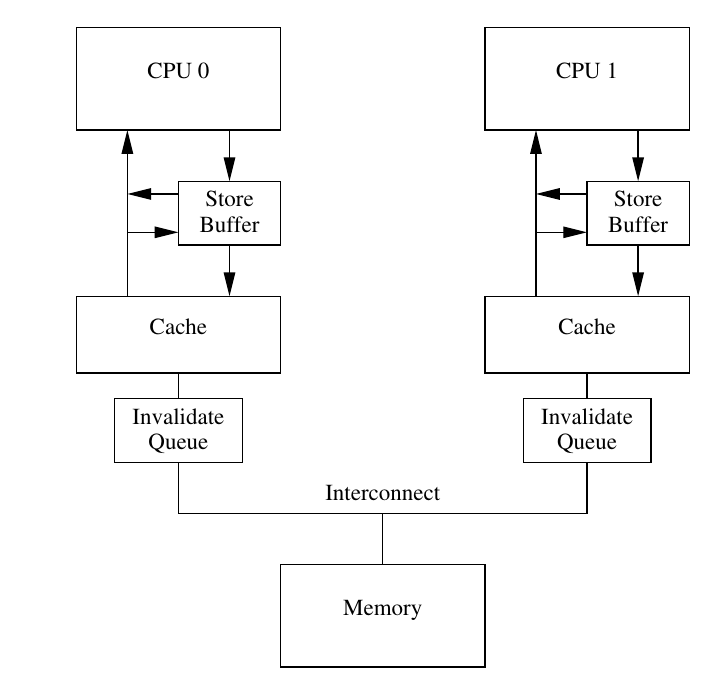
\includegraphics[width=.7\textwidth]{cache-with-wb-iq}

		\end{column}
		
		\begin{column}{.5\textwidth}
			
			\Large
            Cache Coherent in Multi-processor
			\begin{itemize}
				\item  MSI 一致性协议
				\item MESI 一致性协议
			
			\end{itemize}
			
		\end{column}
		
		
	\end{columns}
	
\tiny ref:
Some info are from

Paul McKenney (IBM) Tom Hart (University of Toronto), Frans Kaashoek (MIT), 
Daniel J. Sorin "A Primer on Memory Consistency and Cache Coherence", Fabian Giesen "Cache coherency primer", Mingyu Gao(Tsinghua),Yubin Xia(SJTU)
"The C/C++ Memory Model: Overview and Formalization",Mark Batty,etc. "C++ 11 Memory Consistency Model", Sebastian Gerstenberg;"HOW UBISOFT MONTREAL
DEVELOPS GAMES FOR MULTICORE Before \& After C++11", Jeff Preshing;etc.

	
\end{frame}


%----------------------------------------------
\begin{frame}[plain]	
    \frametitle{Recap}
    
    
    \begin{columns}
        
        \begin{column}{.4\textwidth}
            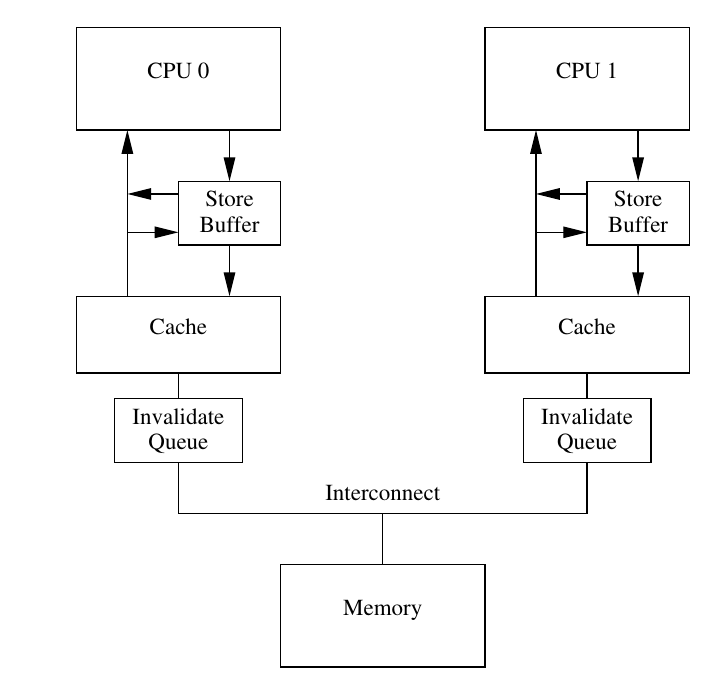
\includegraphics[width=1.\textwidth]{cache-with-wb-iq}
        \end{column}
        \begin{column}{.6\textwidth}
			
\Large
 Memory Consistency in Multi-processor
\begin{itemize}
    \item Sequential Consistency
    \item  Total Store Order Consistency
    \item Acquire/Release Consistency
    
    \item Relaxed/Weak Consistency
    
    
\end{itemize}
        \end{column}
    \end{columns}
    
\end{frame}

%----------------------------------------------
\begin{frame}
    \frametitle{Multiprocessor Programming}

    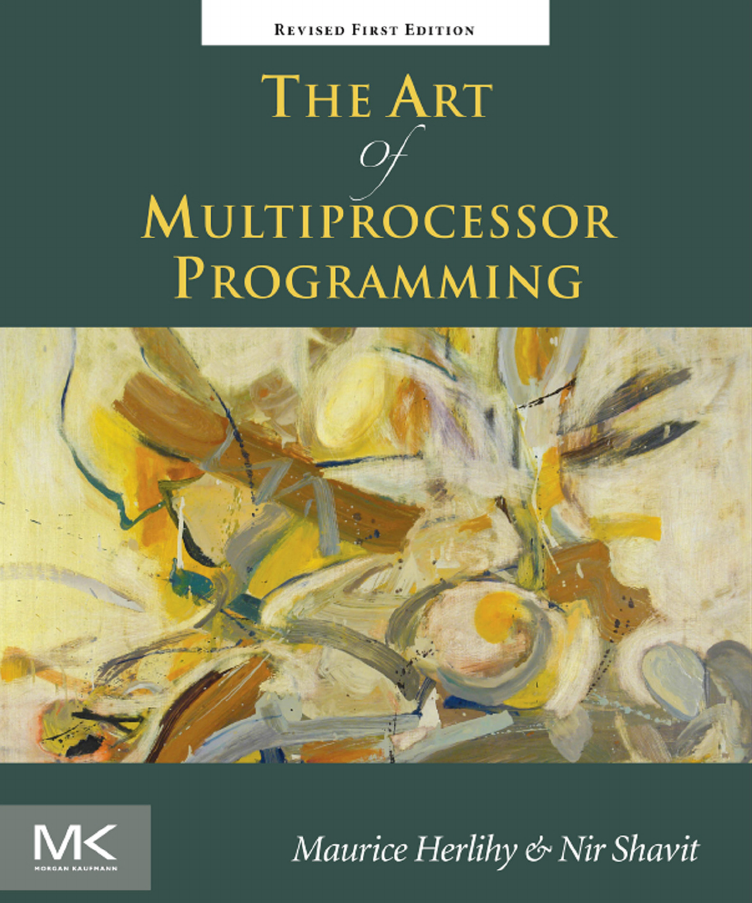
\includegraphics[width=.4\textwidth]{book-the-art-multiprocessor-programming}
    
\includegraphics[width=.385\textwidth]{book-cpp-concurrency-in-action}
\end{frame}


%----------------------------------------------
\begin{frame}
    \frametitle{Ways to Achieve Synchronizes-With}
    C++11/17/20, Go, RUST, Java, ...
    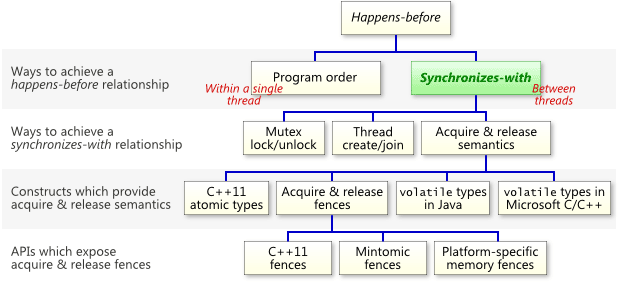
\includegraphics[width=1.\textwidth]{ways-sync}
\end{frame}

%----------------------------------------------
\begin{frame}
  \frametitle{Real Hardware/Compiler}
    Real hardware doesn’t run the code that you wrote.
    
    Real compiler doesn’t produce the code that you wrote.
    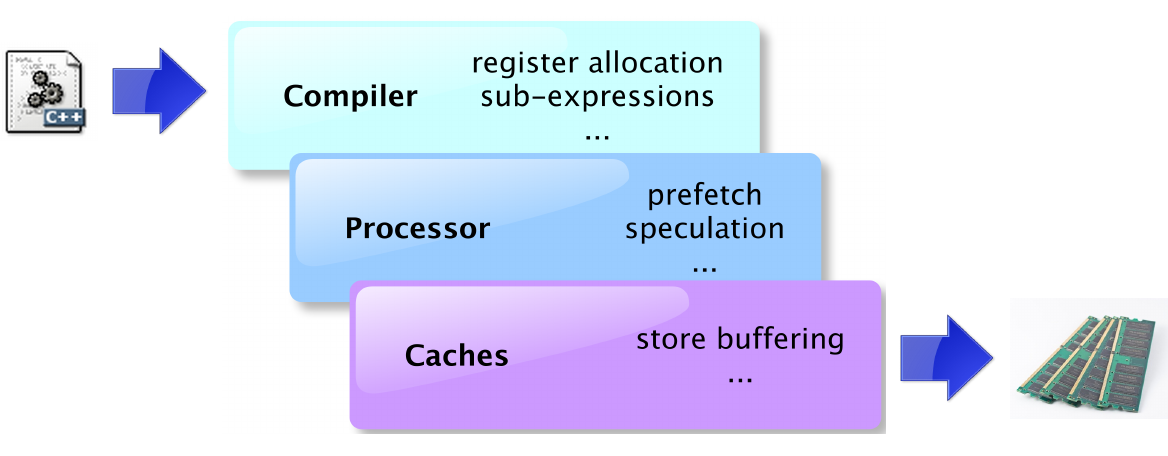
\includegraphics[width=1.\textwidth]{c-compiler-mem-model}
\end{frame}


%----------------------------------------------
\begin{frame}
    \frametitle{Real Hardware/Compiler}
    Real hardware doesn’t run the code that you wrote.
    
    Real compiler doesn’t produce the code that you wrote.
    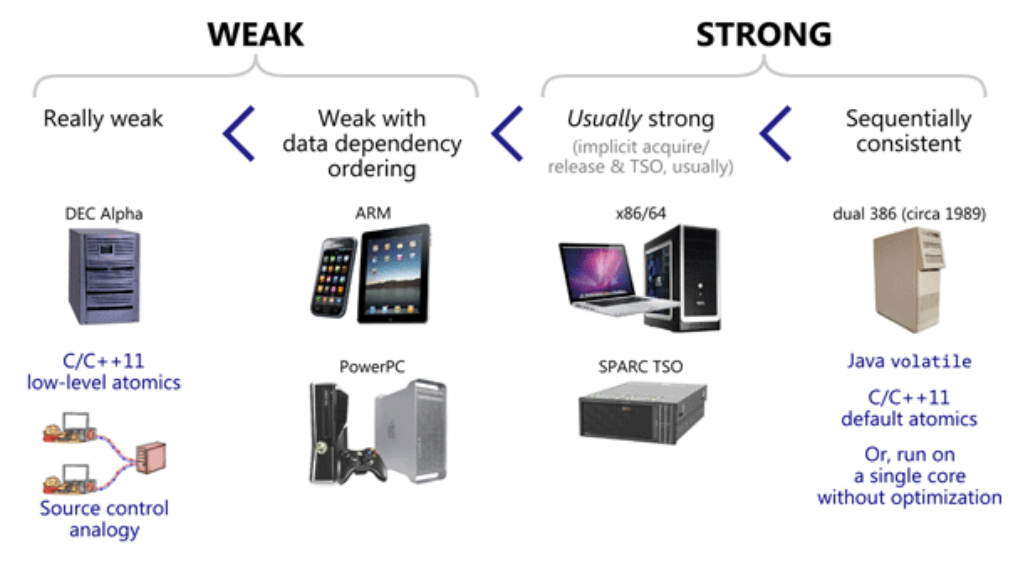
\includegraphics[width=.7\textwidth]{cpu-archs-mem-model}
    
        \tiny
    http://preshing.com/20140709/the-purpose-of-memory\_order\_consume-in-cpp11/
    
%    https://preshing.com/20120612/an-introduction-to-lock-free-programming/
%    在x86 / 64指令级别上,每次从内存中加载都会获取语义,并且每次存储到内存都将提供释放语义–至少对于非SSE指令和非写组合内存。结果,过去写无锁代码在x86 / 64上有效,但在其他处理器上却失败了。
\end{frame}

%----------------------------------------------
\begin{frame}
    \frametitle{Real Hardware/Compiler}
    Real hardware doesn’t run the code that you wrote.
    
    Real compiler doesn’t produce the code that you wrote.
    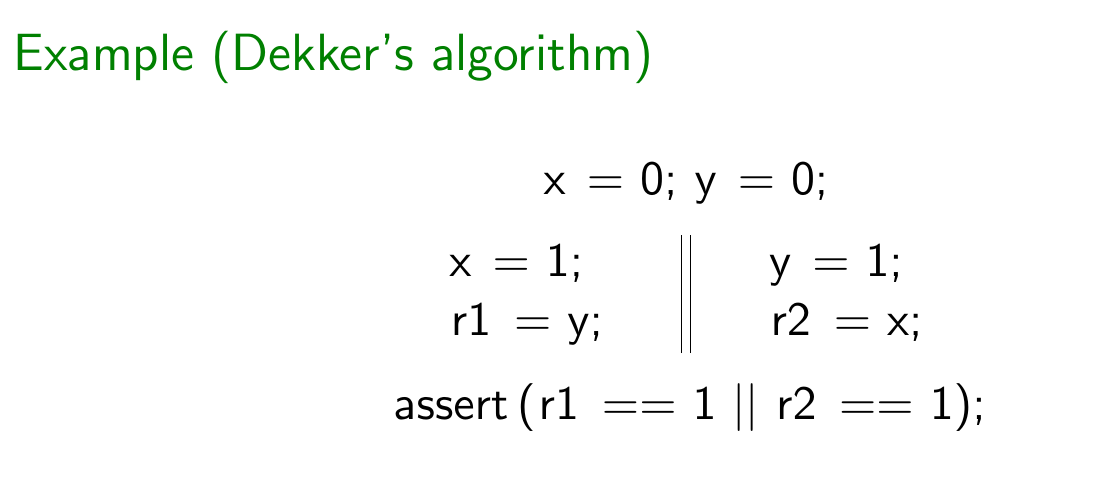
\includegraphics[width=.7\textwidth]{dekker-algorithm}
    
    根据英特尔的规范:在本示例的末尾,r1和r2都等于0是合法的
\end{frame}

%----------------------------------------------
\begin{frame}
    \frametitle{Real Hardware/Compiler}
    Real hardware doesn’t run the code that you wrote.
    
    Real compiler doesn’t produce the code that you wrote.
    
    \centering
    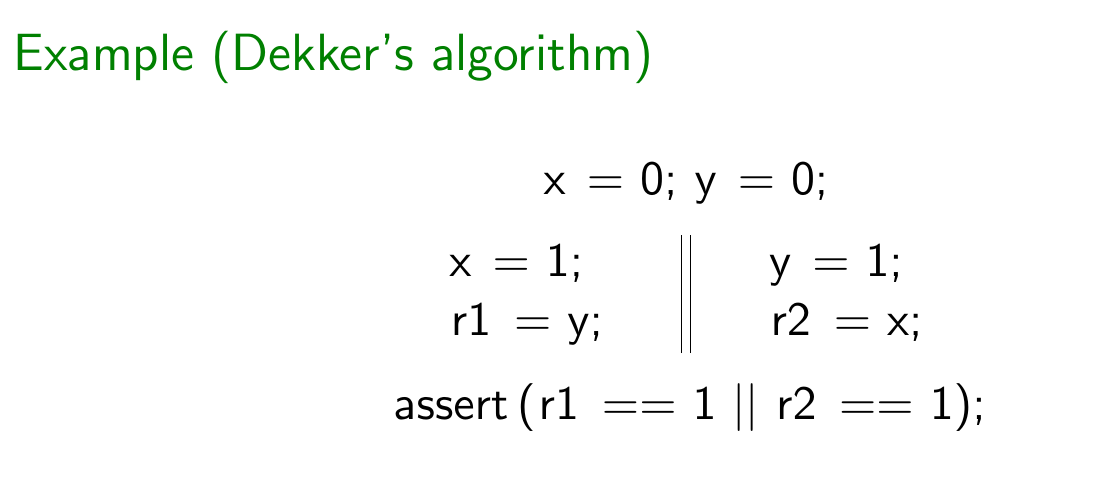
\includegraphics[width=.5\textwidth]{dekker-algorithm}
    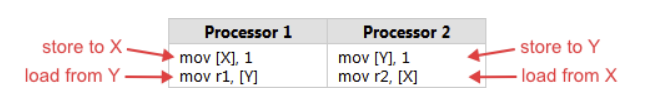
\includegraphics[width=.7\textwidth]{dekker-x86}
\end{frame}

%----------------------------------------------
\begin{frame}
    \frametitle{Real Hardware/Compiler}
    Real hardware doesn’t run the code that you wrote.
    
    Real compiler doesn’t produce the code that you wrote.
    
    \centering
    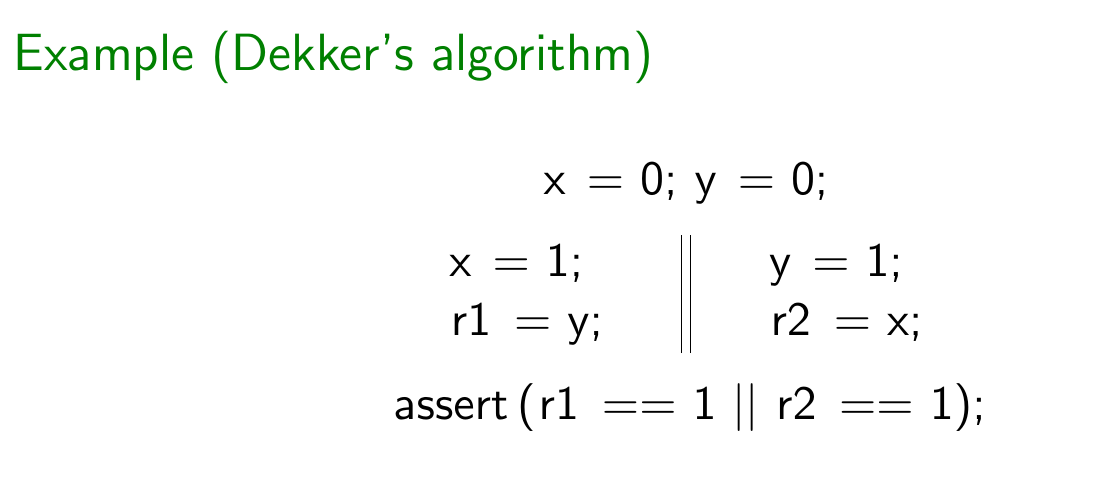
\includegraphics[width=.5\textwidth]{dekker-algorithm}
    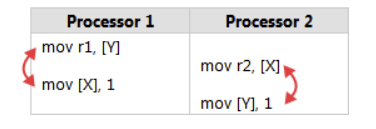
\includegraphics[width=.5\textwidth]{dekker-x86-reorder}
    
    \tiny
    https://preshing.com/20120515/memory-reordering-caught-in-the-act/
\end{frame}

%----------------------------------------------
\begin{frame}
    \frametitle{Real Hardware/Compiler}
    Real hardware doesn’t run the code that you wrote.
    
    Real compiler doesn’t produce the code that you wrote.
    
    \centering
    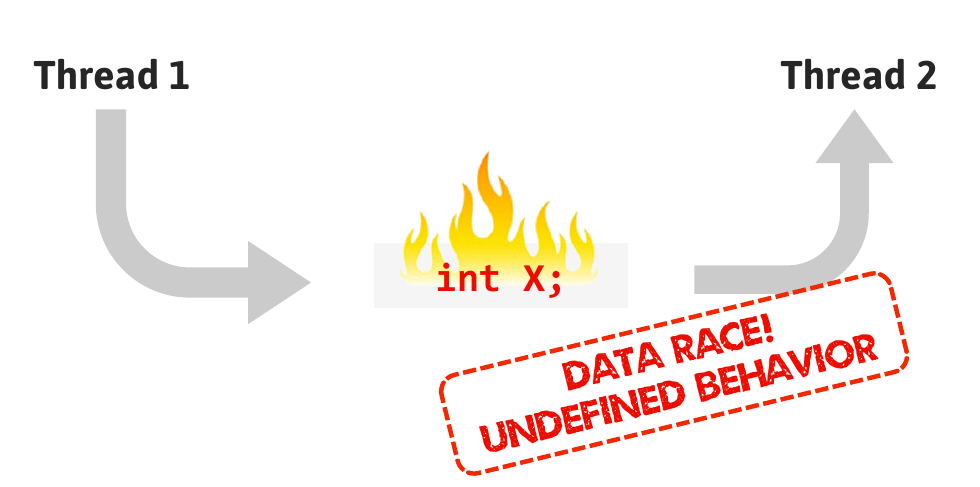
\includegraphics[width=.7\textwidth]{int-x-1}

\end{frame}

%----------------------------------------------
\begin{frame}
    \frametitle{Real Hardware/Compiler}
    Real hardware doesn’t run the code that you wrote.
    
    Real compiler doesn’t produce the code that you wrote.
    
    \centering
    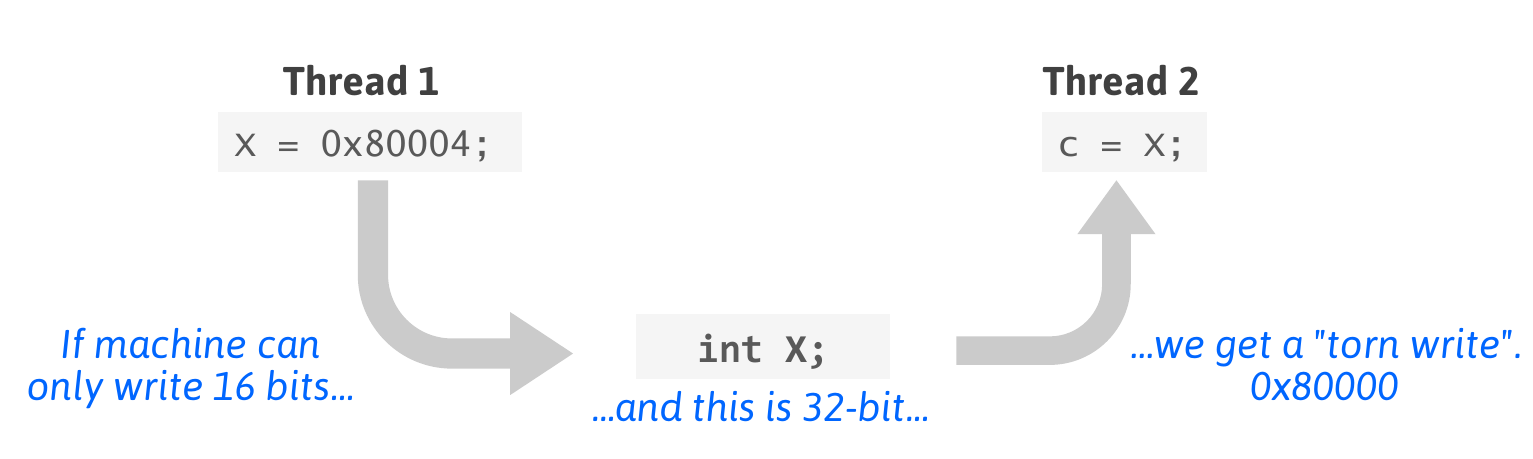
\includegraphics[width=1.\textwidth]{int-x-2-bad}
    
\end{frame}
%----------------------------------------------
\begin{frame}
    \frametitle{Real Hardware/Compiler}
    Real hardware doesn’t run the code that you wrote.
    
    Real compiler doesn’t produce the code that you wrote.
    
    Dekkers Algorithm, g++ -O2
    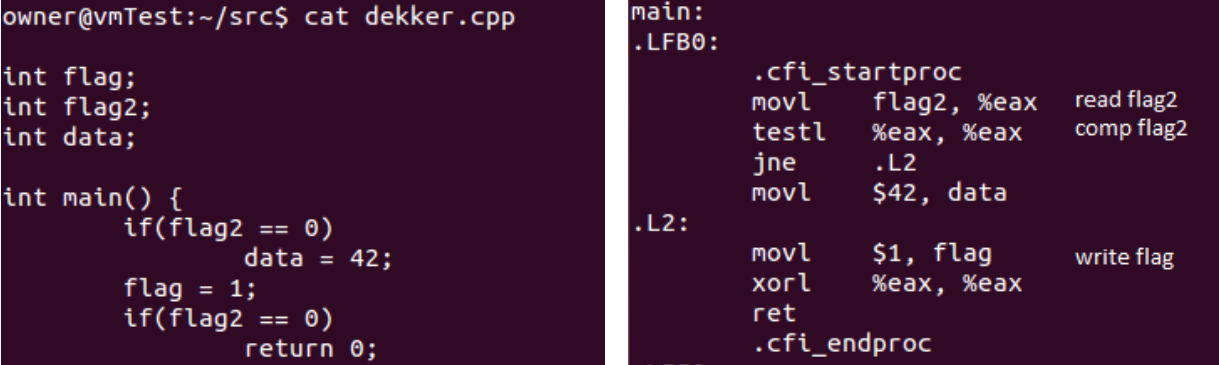
\includegraphics[width=1.\textwidth]{dekker-asm}
\end{frame}
%----------------------------------------------
\begin{frame}
    \frametitle{C++11 Memory Model}
    
    
    \begin{columns}
        
        \begin{column}{.4\textwidth}
            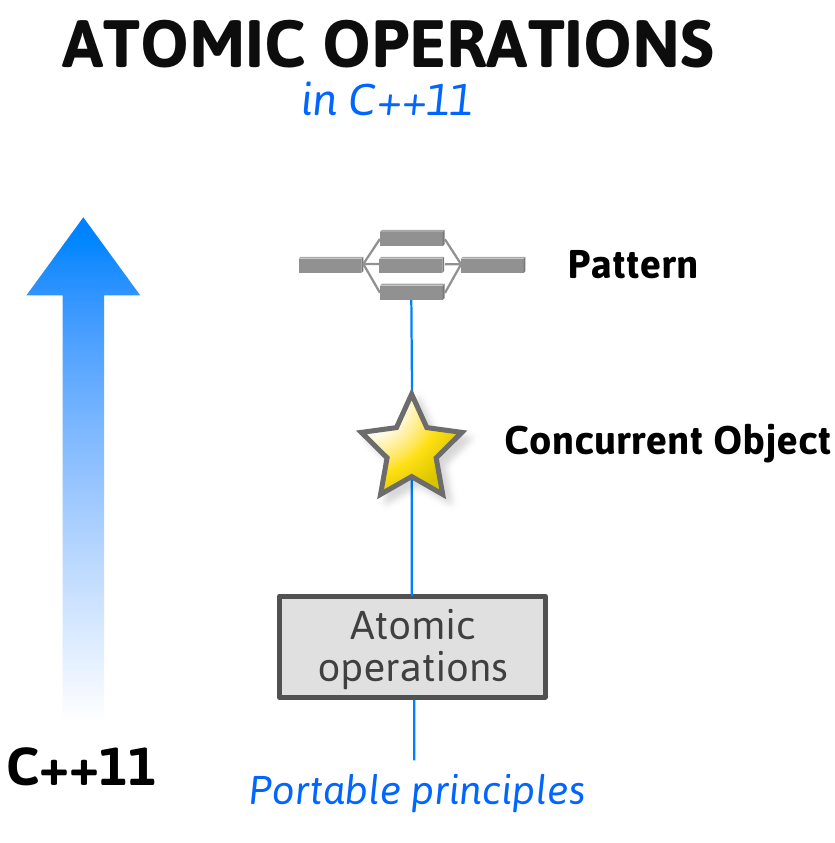
\includegraphics[width=1.\textwidth]{cpp-11}
        \end{column}
        \begin{column}{.6\textwidth}
            
            \Large
            History
            \normalsize
            \begin{itemize}
                \item In 2011, new versions of the ISO standards for C and C++,
                informally known as C11 and C++11, were ratified.
                
                \item These standards define a memory model for C/C++
                \item Support for this model has recently become available in popular
                compilers (GCC 4.4, Intel C++ 13.0, MSVC 11.0, Clang 3.1).
                
                
                
            \end{itemize}
        \end{column}
    \end{columns}
    
\end{frame}


%----------------------------------------------
\begin{frame}
    \frametitle{C++11 Memory Model}
    
    
    \begin{columns}
        
        \begin{column}{.4\textwidth}
            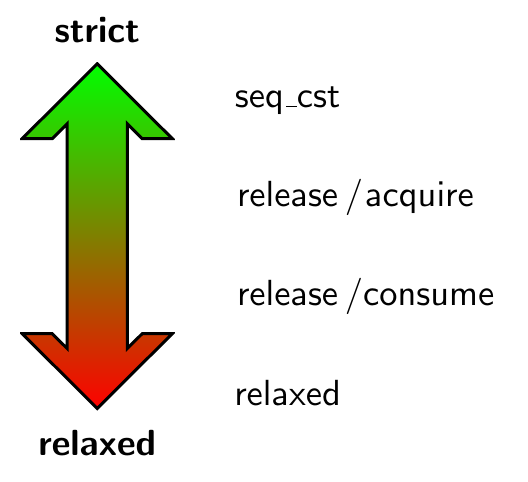
\includegraphics[width=1.\textwidth]{cpp-mem-model}
        \end{column}
        \begin{column}{.6\textwidth}
            
            \Large
            Why C++11 Memory Model
            \normalsize
            \begin{itemize}
                \item 在C++11之前,其实是没有定义内存模型的,我们所使用的都是一些处理器/编译器暴露的同步原语,比如 GCC 的内联汇编,内建函数之类的,有着不同的实现。
                \item C++11在标准库中引入了memory model的意义在于在High Level Language层面实现对在多处理器中多线程共享内存的访问,实现跨编译器,OS和硬件的差异性。

                
                
            
                
            \end{itemize}
        \end{column}
    \end{columns}
    
\end{frame}


%----------------------------------------------
\begin{frame}
    \frametitle{C++11 Memory Model}
    
    
    \begin{columns}
        
        \begin{column}{.4\textwidth}
            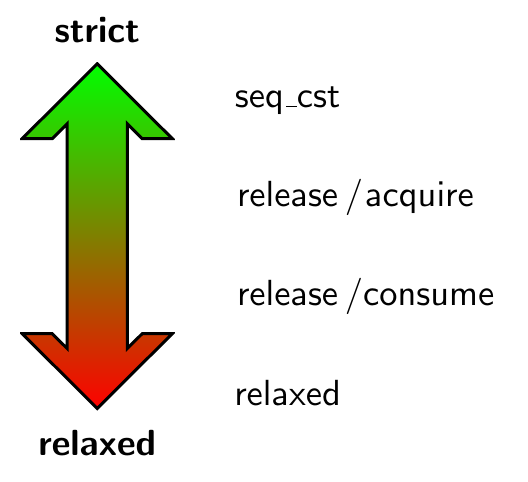
\includegraphics[width=1.\textwidth]{cpp-mem-model}
        \end{column}
        \begin{column}{.6\textwidth}
            
            \Large
            Happens-before
            \normalsize
            \begin{itemize}
                \item An important fundamental concept in understanding the
                memory model
                
                \item A guarantee that memory writes by one specific
                statement are visible to another specific statement
                
                
            \end{itemize}
            

        \end{column}
    \end{columns}
    
\end{frame}


%----------------------------------------------
\begin{frame}[fragile]
    \frametitle{C++11 Memory Model}
    \LARGE
    Happens-before
    %    \normalsize
    \large    
    \begin{block}{}
        \begin{verbatim}
int A = 0;
int B = 0;

void foo()
{
    A = B + 1;              // (1)
    B = 1;                  // (2)
}
\end{verbatim}
    \end{block}
    
\end{frame}

%----------------------------------------------
\begin{frame}[fragile]
    \frametitle{C++11 Memory Model}
    \LARGE
    Happens-before
    
        \centering    
   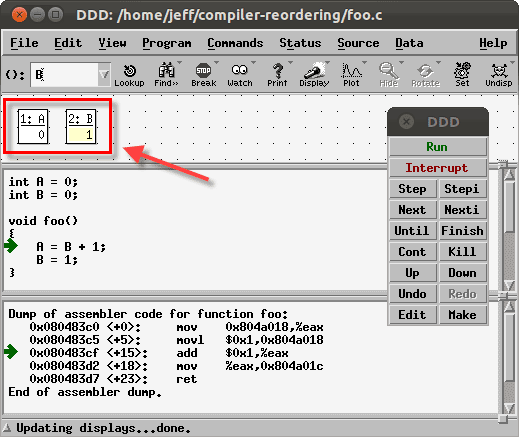
\includegraphics[width=.5\textwidth]{happen-before-debug}
    
\end{frame}
%----------------------------------------------
\begin{frame}[fragile]
    \frametitle{C++11 Memory Model}
    \LARGE
     Happens-before
%    \normalsize
\large    
    \begin{block}{}
        \begin{verbatim}
    int A, B;
    
    void foo()
    {
        A = B + 1;
        B = 0;
    }
\end{verbatim}
    \end{block}
    
\end{frame}


%----------------------------------------------
\begin{frame}[fragile]
    \frametitle{C++11 Memory Model}
    \LARGE
    Happens-before
    %    \normalsize
    \large    
    
    GCC 4.6.1
    \begin{block}{}
        \begin{verbatim}
$ gcc -S -masm=intel foo.c
$ cat foo.s
    ...
    mov     eax, DWORD PTR _B  (redo this at home...)
    add     eax, 1
    mov     DWORD PTR _A, eax
    mov     DWORD PTR _B, 0
    ...
        \end{verbatim}
    \end{block}
    
\end{frame}

%----------------------------------------------
\begin{frame}[fragile]
    \frametitle{C++11 Memory Model}
    \LARGE
    Happens-before
    %    \normalsize
    \large    
    
    GCC 4.6.1
    \begin{block}{}
        \begin{verbatim}
$ gcc -O2 -S -masm=intel foo.c
$ cat foo.s
    ...
    mov     eax, DWORD PTR B
    mov     DWORD PTR B, 0
    add     eax, 1
    mov     DWORD PTR A, eax
    ...
        \end{verbatim}
    \end{block}
    
\end{frame}


%----------------------------------------------
\begin{frame}[fragile]
    \frametitle{C++11 Memory Model}
    \LARGE
    Happens-before
    %    \normalsize
    \large    
    
    GCC 4.6.1
    \begin{block}{}
        \begin{verbatim}
    int A, B;
    
    void foo()
    {
        A = B + 1;
        asm volatile("" ::: "memory");
        B = 0;
    }
        \end{verbatim}
    \end{block}
    
\end{frame}


%----------------------------------------------
\begin{frame}[fragile]
    \frametitle{C++11 Memory Model}
    \LARGE
    Happens-before
    %    \normalsize
    \large    
    
    GCC 4.6.1
    \begin{block}{}
        \begin{verbatim}
$ gcc -O2 -S -masm=intel foo.c
$ cat foo.s
    ...
    mov     eax, DWORD PTR _B
    add     eax, 1
    mov     DWORD PTR _A, eax
    mov     DWORD PTR _B, 0
    ...
        \end{verbatim}
    \end{block}
    
\end{frame}


%----------------------------------------------
\begin{frame}[fragile]
    \frametitle{C++11 Memory Model}
    \LARGE
    Happens-before
    %    \normalsize
    \large    
    \begin{block}{}
        \begin{verbatim}
//x86
#define COMPILER_BARRIER() asm volatile("" ::: "memory") 
//PowerPC
#define RELEASE_FENCE() asm volatile("lwsync" ::: "memory") 
==============================================
int Value;
std::atomic<int> IsPublished(0);
void sendValue(int x)
{
    Value = x;
    // <-- reordering is prevented here!
    IsPublished.store(1, std::memory_order_release);
}
\end{verbatim}
    \end{block}
    
\end{frame}
%----------------------------------------------
\begin{frame}
    \frametitle{C++11 Memory Model}
    
    
    \begin{columns}
        
        \begin{column}{.4\textwidth}
            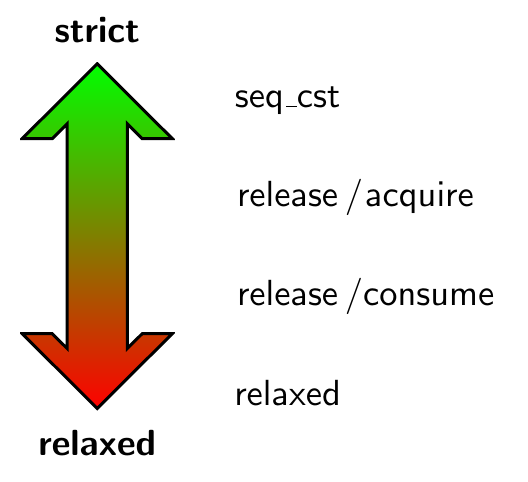
\includegraphics[width=1.\textwidth]{cpp-mem-model}
        \end{column}
        \begin{column}{.6\textwidth}
            
            \Large
            std :: atomic<T>

            \begin{itemize}
                \item x.load(memory order)
                \item x.store (T, memory order)
                
            \end{itemize}
         \normalsize
        Concurrent accesses on atomic locations do not race.
        
        The memory order argument specifies ordering constraints between
        atomic and non-atomic memory accesses in different threads.
                    
        \end{column}
    \end{columns}
    
    \end{frame}


%----------------------------------------------
\begin{frame}
    \frametitle{C++11 Memory Model}
    \Large
    If multiple threads access the same variable concurrently, and at least one
    thread modifies it, all threads must use C++11 atomic operations.
    
    \centering
    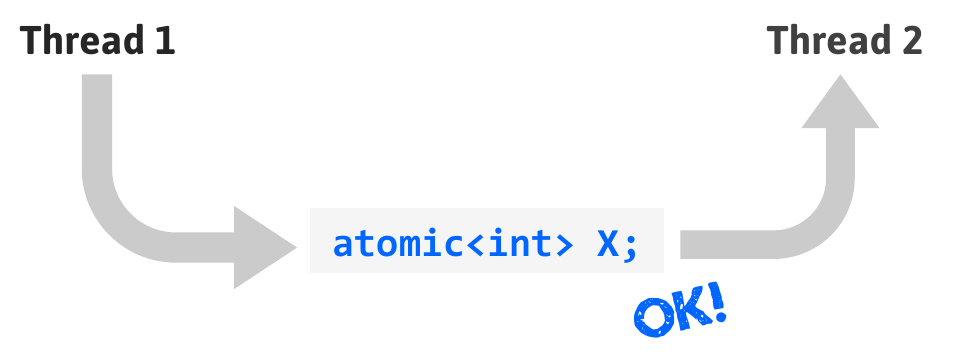
\includegraphics[width=.8\textwidth]{atomic-int-x}
\end{frame}

%----------------------------------------------
\begin{frame}
    \frametitle{C++11 Memory Model}
    \LARGE
    std :: atomic<T>
    
    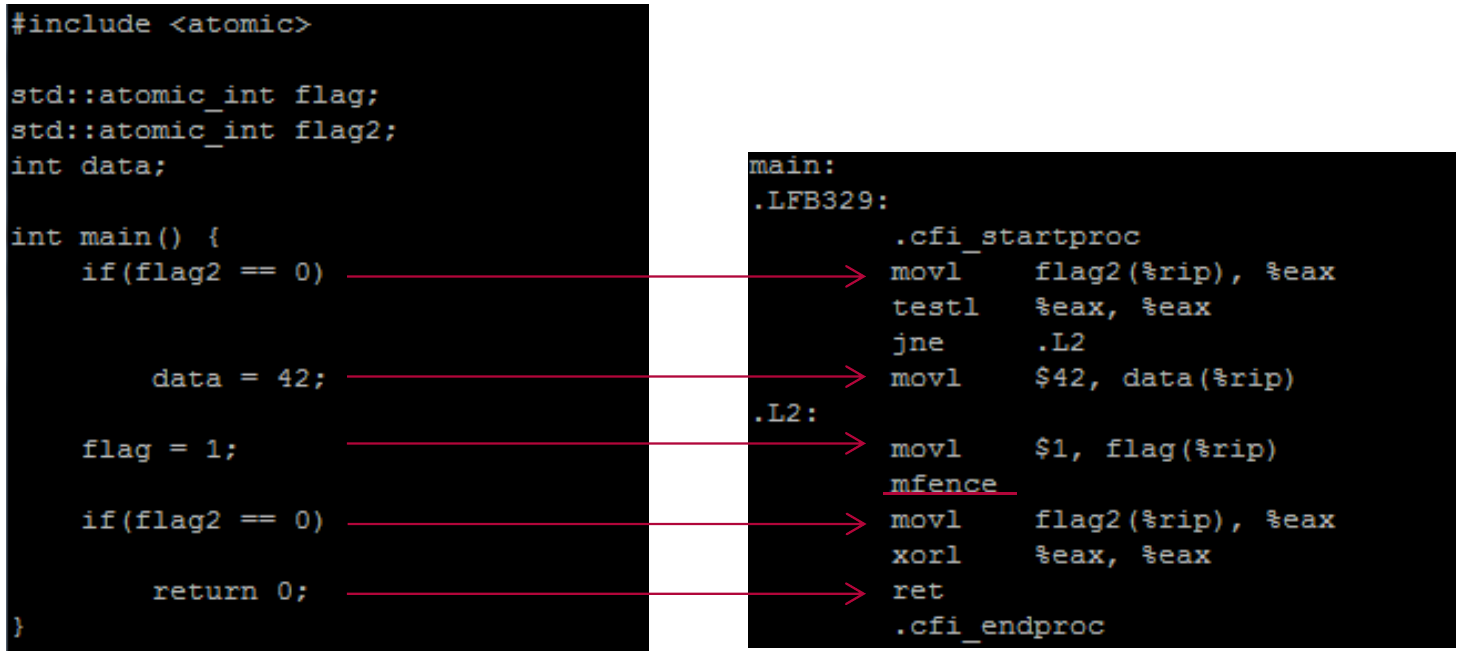
\includegraphics[width=.8\textwidth]{atomic-asm}
\end{frame}

%----------------------------------------------
\begin{frame}
    \frametitle{C++11 Memory Model}
    \LARGE
    std :: atomic<T>
    
    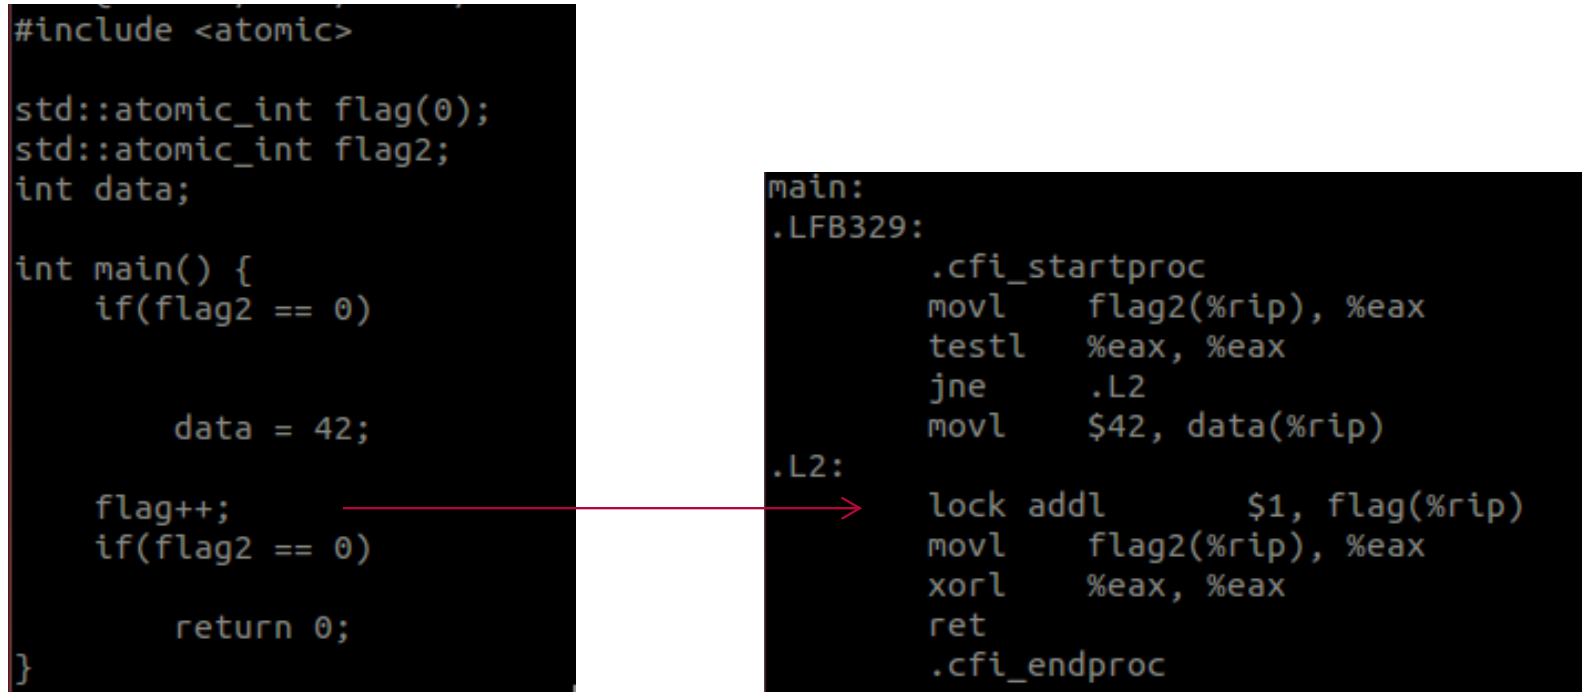
\includegraphics[width=.8\textwidth]{atomic-asm2}
\end{frame}
%----------------------------------------------
\begin{frame}
    \frametitle{C++11 Memory Model}
    \LARGE
    std :: memory\_order
    
    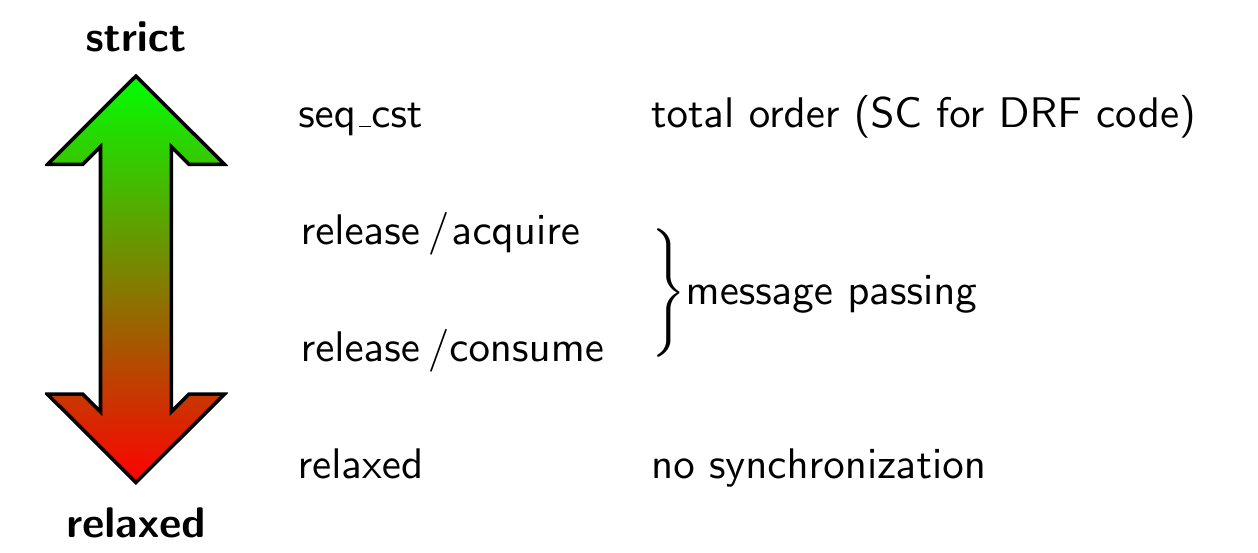
\includegraphics[width=1.\textwidth]{cpp-all-mem-order}
\end{frame}


%----------------------------------------------
\begin{frame}
    \frametitle{C++11 Memory Model}
    \LARGE
    std :: memory\_order\_seq\_cst
    
    \normalsize
    There is a total order over all seq cst operations. This order
    contributes to inter-thread ordering constraints.
    
    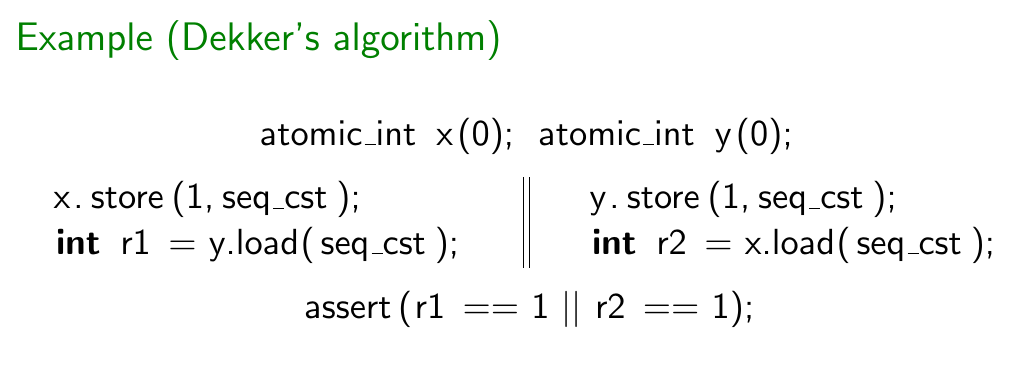
\includegraphics[width=1.\textwidth]{dekker-seq-order}
\end{frame}



%----------------------------------------------
\begin{frame}
    \frametitle{C++11 Memory Model}
    \LARGE
    std :: memory\_order\_seq\_cst
    
    %    \normalsize
    %    There is a total order over all seq cst operations. This order
    %    contributes to inter-thread ordering constraints.
    \centering
    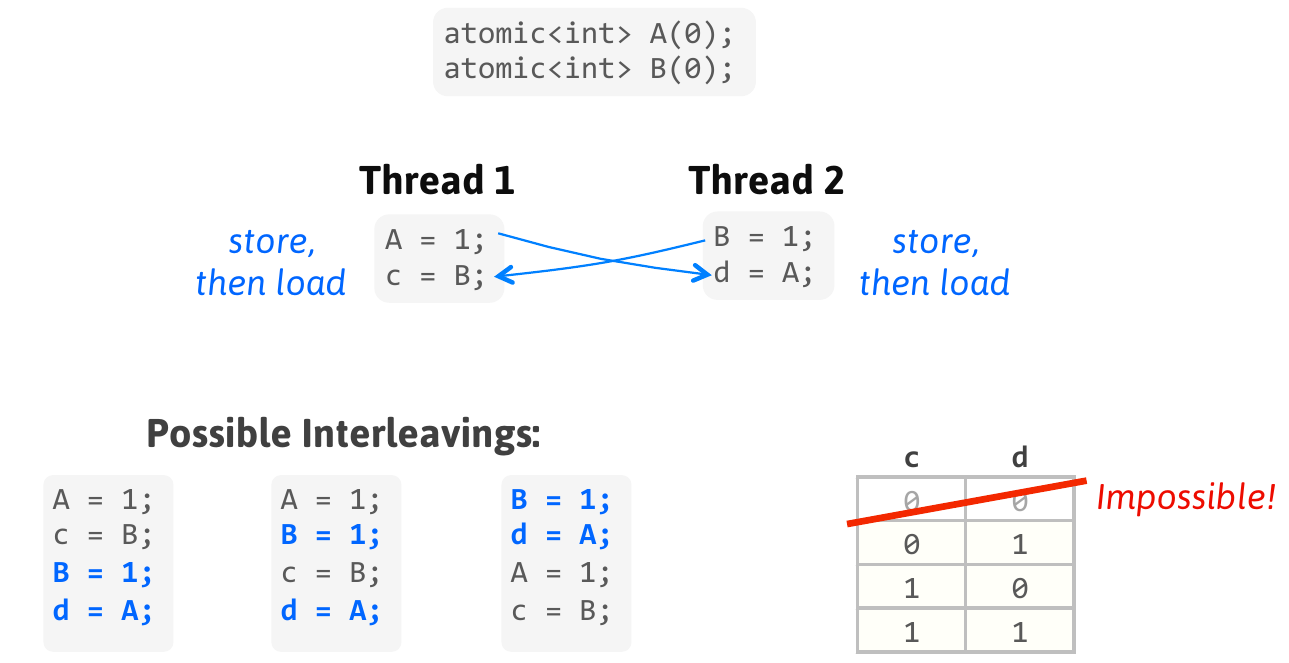
\includegraphics[width=.8\textwidth]{seq-order}
\end{frame}


%----------------------------------------------
\begin{frame}
    \frametitle{C++11 Memory Model}
    \LARGE
    std :: memory\_order\_seq\_cst
    
    
    sequential consistency
    
    \normalsize
    直观上,读操作应该返回“最后”一次写入的值。
    \begin{itemize}
        \item 在单处理器系统中,“最后”由程序次序定义。
        \item 在多处理器系统中,我们称之为顺序连贯(sequential consistency, SC).
    \end{itemize}
    约束条件
    \begin{itemize}
        \item 在每个处理器内,维护每个处理器的程序次序;
        \item 在所有处理器间,维护单一的表征所有操作的次序。对于写操作W1, W2, 不能出现从处理器 P1 看来,执行次序为 W1->W2; 从处理器 P2 看来,执行次序却为 W2->W1 这种情况。 
    \end{itemize}
    
\end{frame}

%----------------------------------------------
\begin{frame}
    \frametitle{C++11 Memory Model}
    \LARGE
    std :: memory\_order\_release/acquire
    
    \normalsize
    An acquire load makes prior writes to other memory locations
    made by the thread that did the release visible in the loading
    thread.
    
    
    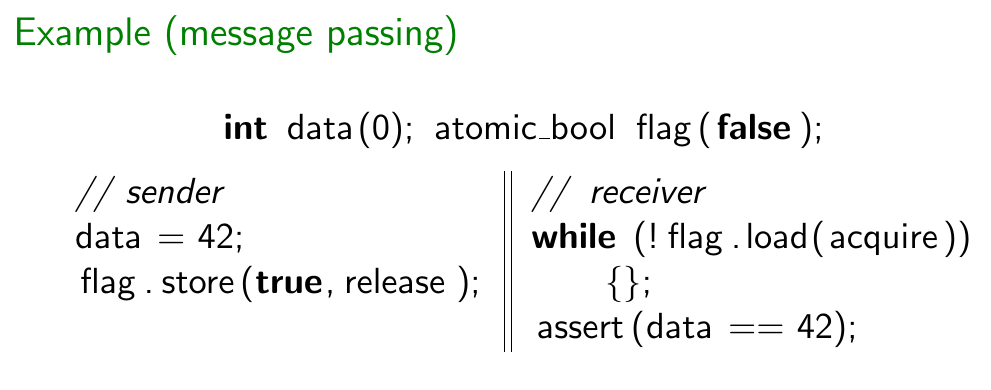
\includegraphics[width=.8\textwidth]{dekker-acrel-order}
\end{frame}

%----------------------------------------------
\begin{frame}
    \frametitle{C++11 Memory Model}
    \LARGE
    std :: memory\_order\_release/acquire
    
    \normalsize
    An acquire load makes prior writes to other memory locations
    made by the thread that did the release visible in the loading
    thread.
    
    
    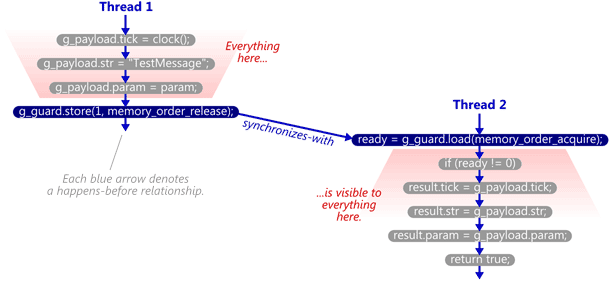
\includegraphics[width=.8\textwidth]{acrel-pic}
\end{frame}

%----------------------------------------------
\begin{frame}
    \frametitle{C++11 Memory Model}
    \LARGE
    std :: memory\_order\_release/acquire
    
    \large
\begin{block}{Acquire semantics}
    
Acquire semantics is a property that can only apply to operations that read from shared memory, whether they are read-modify-write operations or plain loads. The operation is then considered a \textbf{read-acquire}. Acquire semantics prevent memory reordering of the read-acquire with any read or write operation that follows it in program order.
\end{block}
%\includegraphics[width=.3\textwidth]{read-require}
    \end{frame}

%----------------------------------------------
\begin{frame}
    \frametitle{C++11 Memory Model}
    \LARGE
    std :: memory\_order\_release/acquire
    
    \large
    \begin{block}{Release semantics}
        
Release semantics is a property that can only apply to operations that write to shared memory, whether they are read-modify-write operations or plain stores. The operation is then considered a write-release. Release semantics prevent memory reordering of the write-release with any read or write operation that precedes it in program order.
    \end{block}
    %\includegraphics[width=.3\textwidth]{read-require}
\end{frame}


%----------------------------------------------
\begin{frame}
    \frametitle{C++11 Memory Model}
    \LARGE
    std :: memory\_order\_release/acquire
    
    \centering
    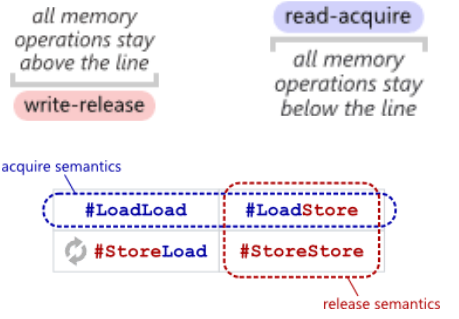
\includegraphics[width=.6\textwidth]{acq-rel}
\end{frame}


%----------------------------------------------
\begin{frame}[fragile]
    \frametitle{C++11 Memory Model}
    \LARGE
    std :: memory\_order\_release/acquire
\normalsize    
\begin{block}{}
    \begin{verbatim}
void produce() {
    payload = 42;
    guard.store(1, std::memory_order_release)
}
void consume(int iterations) {
    for(int i = 0; i < iterations; i++){
      if(guard.load(std::memory_order_acquire))
        result[i] = payload;
    }
}
\end{verbatim}
\end{block}

\end{frame}


%----------------------------------------------
\begin{frame}
    \frametitle{C++11 Memory Model}
    \LARGE
    std :: memory\_order\_release/acquire
    
    
    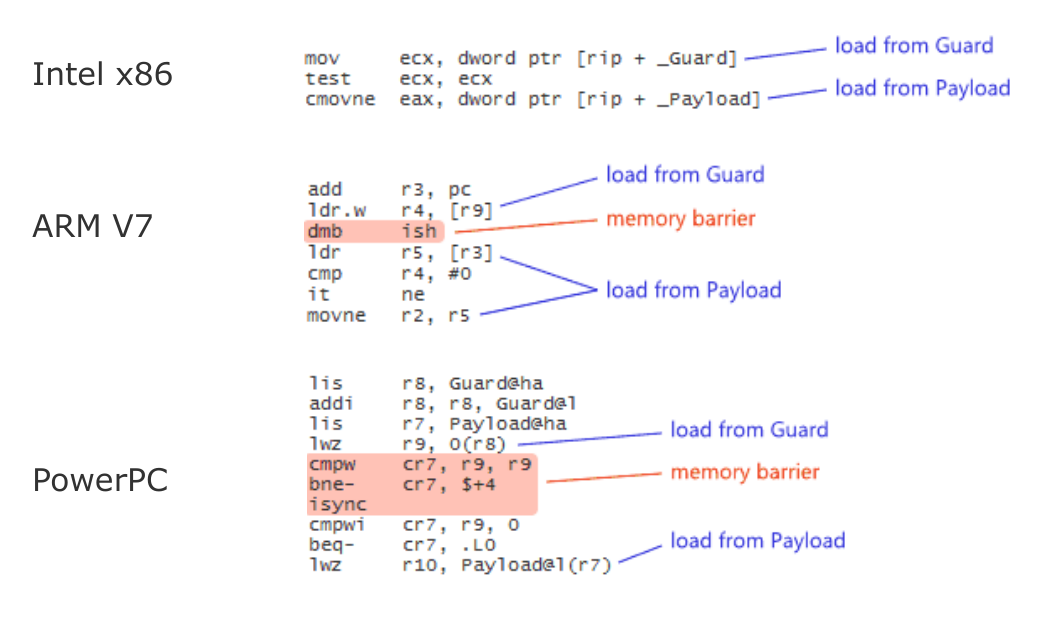
\includegraphics[width=.7\textwidth]{acrel-asm}
    \tiny
    http://preshing.com/20140709/the-purpose-of-memory\_order\_consume-in-cpp11/
    
\end{frame}

%----------------------------------------------
\begin{frame}
    \frametitle{C++11 Memory Model}
    \LARGE
    std :: memory\_order\_release/acquire
%    \normalsize
    
    1000 iterations:
    
    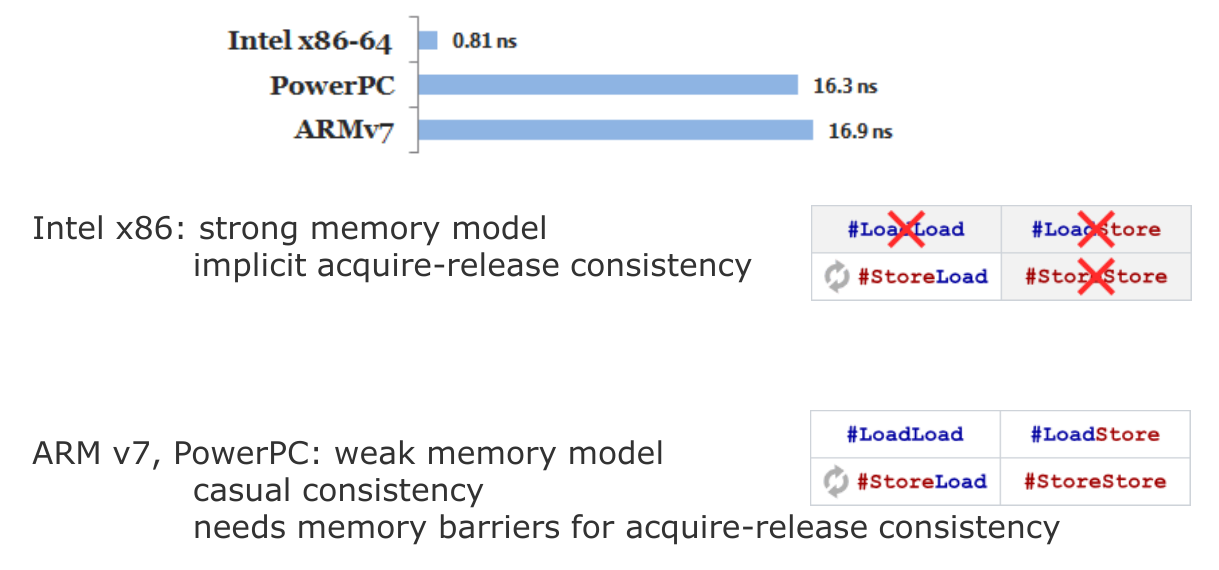
\includegraphics[width=.8\textwidth]{acrel-perf}
    \tiny
    http://preshing.com/20140709/the-purpose-of-memory\_order\_consume-in-cpp11/
    
\end{frame}

%----------------------------------------------
\begin{frame}
    \frametitle{C++11 Memory Model}
    %    https://preshing.com/20140709/the-purpose-of-memory_order_consume-in-cpp11/
    \LARGE
    std :: memory\_order\_consume
    
    
    \normalsize
    (\textbf{Data Dependency Ordering})A consume load makes prior writes to data-dependent memory
    locations made by the thread that did the release visible in the
    loading thread.
    
    \LARGE
    \centering
    \textbf{Data Dependency}
    
    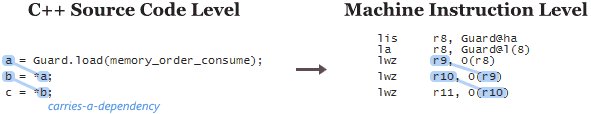
\includegraphics[width=1.\textwidth]{data-depend}
    

\end{frame}


%----------------------------------------------
\begin{frame}
    \frametitle{C++11 Memory Model}
    \LARGE
    std :: memory\_order\_consume
    
    
    \normalsize
    (\textbf{Data Dependency Ordering})A consume load makes prior writes to data-dependent memory
    locations made by the thread that did the release visible in the
    loading thread.
    
    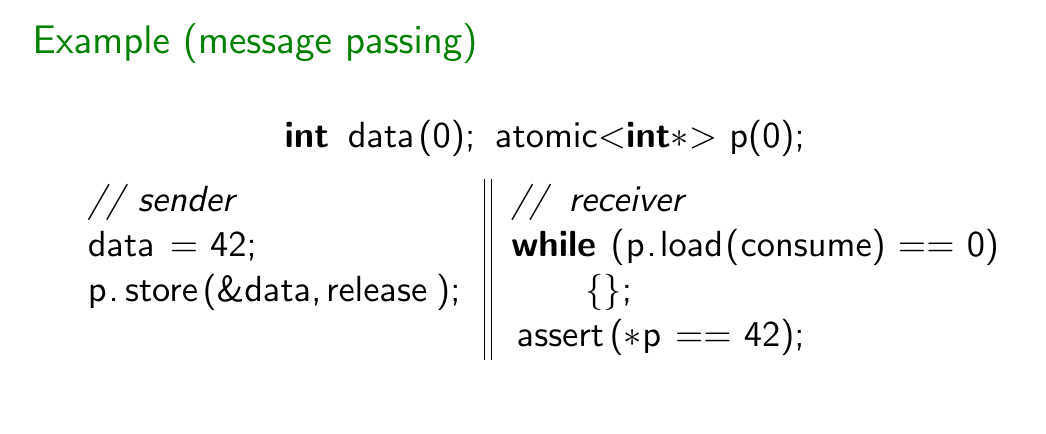
\includegraphics[width=1.\textwidth]{dekker-consume-order}
\end{frame}


%----------------------------------------------
\begin{frame}
    \frametitle{C++11 Memory Model}
    \LARGE
    std :: memory\_order\_consume
    
    
    \normalsize
    (\textbf{Data Dependency Ordering})A consume load makes prior writes to data-dependent memory
    locations made by the thread that did the release visible in the
    loading thread.
    
    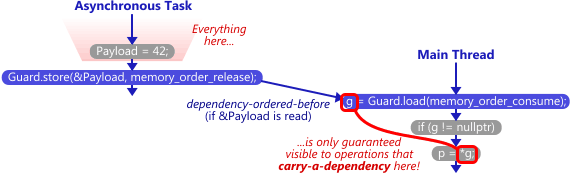
\includegraphics[width=1.\textwidth]{consume-order}
\end{frame}


%----------------------------------------------
\begin{frame}
    \frametitle{C++11 Memory Model}
    \LARGE
    std :: memory\_order\_consume
    
    
    \large
    \begin{itemize}
        \item x86-64 machine code loads Guard into register rcx, then, if rcx is not null, uses rcx to load the payload, thus creating a data dependency between the two load instructions. 
        \item 86-64’s strong memory model already guarantees that loads are performed in-order, even if there isn’t a data dependency.
    \end{itemize}



    
    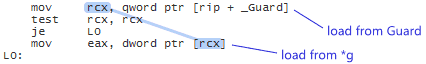
\includegraphics[width=1.\textwidth]{consume-x86}
\end{frame}

%----------------------------------------------
\begin{frame}
    \frametitle{C++11 Memory Model}
    \LARGE
    std :: memory\_order\_consume
    
    
    \large
    \begin{itemize}
        \item PowerPC machine code loads Guard into register r9, then uses r9 to load the payload, thus creating a data dependency between the two load instructions. 
        \item completely avoid the "\textit{\textbf{cmp;bne;isync}}" sequence of instructions that formed a memory barrier in the original example, while still ensuring that the two loads are performed in-order.
    \end{itemize}

    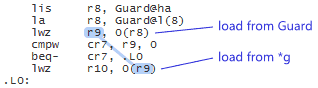
\includegraphics[width=.8\textwidth]{consume-ppc}
\end{frame}

%----------------------------------------------
\begin{frame}
    \frametitle{C++11 Memory Model}
    \LARGE
    std :: memory\_order\_consume
    
    
    \large
    \begin{itemize}
        \item ARMV7 machine code loads Guard into register r4, then uses r4 to load the payload, thus creating a data dependency between the two load instructions.  
        \item completely avoid the "\textbf{\textit{dmb ish }}" instruction that was present in the original example, while still ensuring that the two loads are performed in-order.
    \end{itemize}
    
    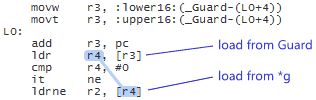
\includegraphics[width=.8\textwidth]{consume-armv7}
\end{frame}
%----------------------------------------------
\begin{frame}
    \frametitle{C++11 Memory Model}
    \LARGE
    std :: memory\_order\_consume
    
    
    \normalsize
    (\textbf{Data Dependency Ordering})A consume load makes prior writes to data-dependent memory
    locations made by the thread that did the release visible in the
    loading thread.
    
    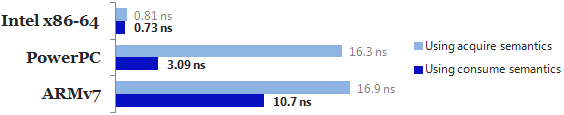
\includegraphics[width=1.\textwidth]{consume-order-perf}
\end{frame}

%----------------------------------------------
\begin{frame}
    \frametitle{C++11 Memory Model}
    \LARGE
    std :: memory\_order\_consume
   
   \normalsize
   \begin{block}{real world -- RCU}
    在真实世界中使用这一技术--利用数据依赖顺序以避免内存栅栏的例子就是Linux内核。Linux提供了读-复制-更新(RCU)的同步机制,适合构建在多个线程中需要多读少写的共享变量(包括指针等)数据结构。Linux实际上没有使用C++11消费语义来去除那些内存栅栏,而是依靠它自己的API和规范。其实起初RCU就被看作是给C++11添加消费语义的动机。  
    \end{block} 
 
\end{frame}
%----------------------------------------------
\begin{frame}
    \frametitle{C++11 Memory Model}
    \LARGE
    std :: memory\_order\_relaxed
    
    
    \normalsize
   The memory\_order\_relaxed ensure these operations are atomic, but don’t impose any ordering constraints/memory barriers that aren’t already there.
   
    relaxed order允许单线程上不同的memory location进行reorder,但是对于同一个memory location不能进行reorder。
    
    \centering
    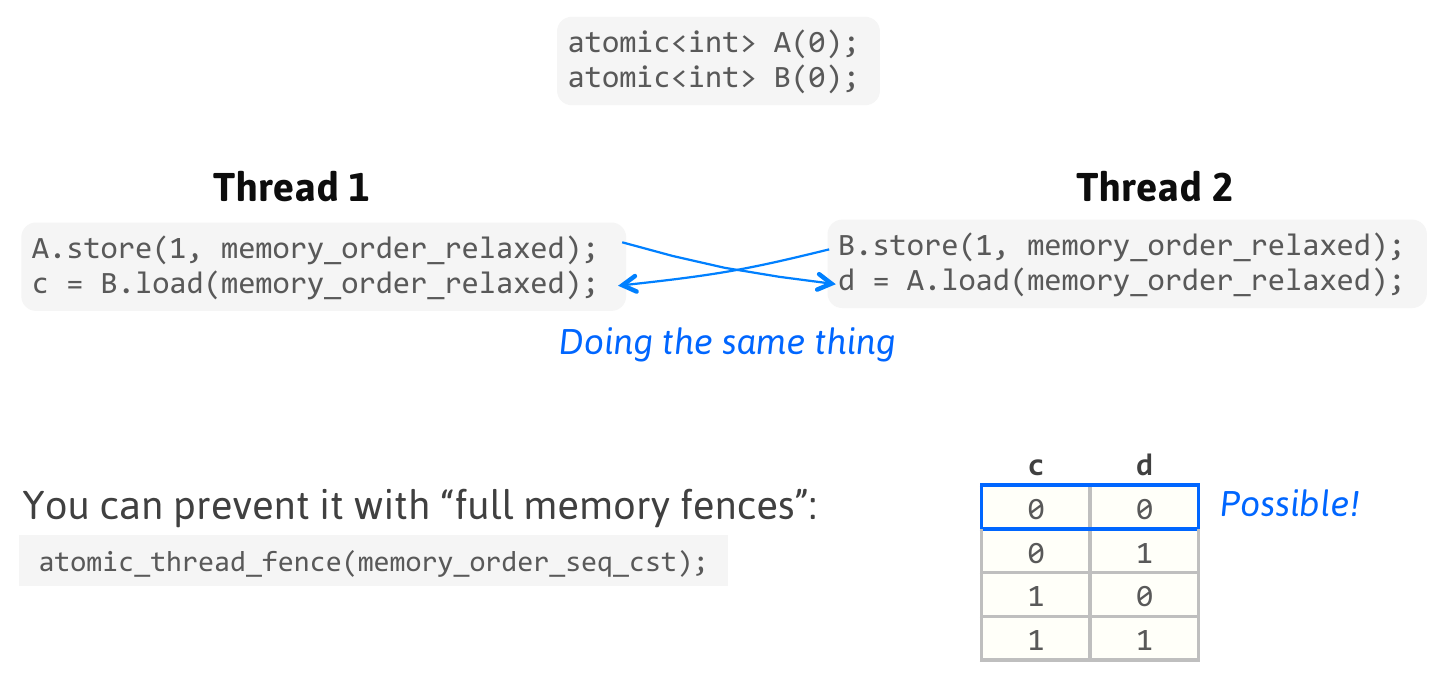
\includegraphics[width=.7\textwidth]{relax-order}
\end{frame}


%----------------------------------------------
\begin{frame}[fragile]
    \frametitle{Lock-Free Programming}
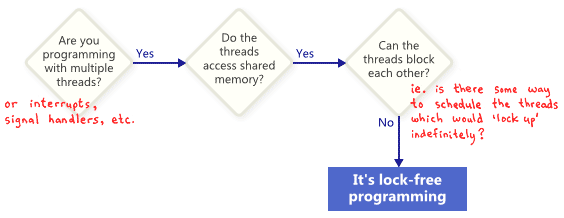
\includegraphics[width=1.\textwidth]{its-lock-free}
    
\end{frame}

%----------------------------------------------
\begin{frame}[fragile]
    \frametitle{Lock-Free Programming}
    
   \centering 
   
    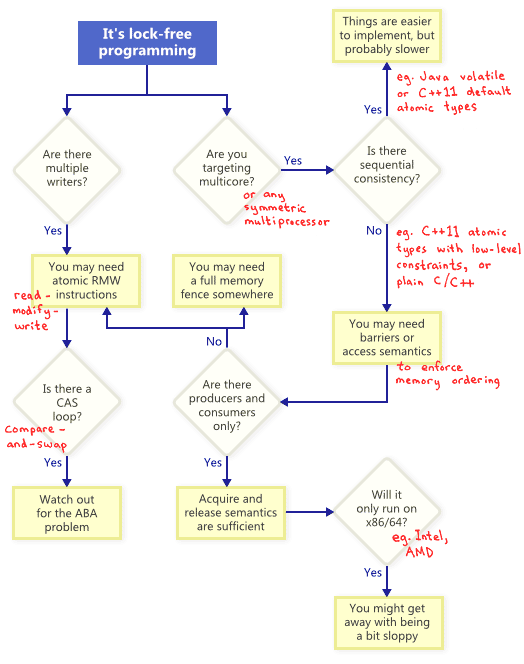
\includegraphics[width=.4\textwidth]{lock-free-tech}
%    https://preshing.com/20120612/an-introduction-to-lock-free-programming/
\end{frame}

%----------------------------------------------
\begin{frame}[fragile]
    \frametitle{Lock-Free Programming}
    \LARGE
    Lock-free Stack
    \normalsize    
    \begin{block}{}
        \begin{verbatim}
template<typename T>
class lock_free_stack
{
    private:
        struct node
        {
            T data;
            node* next;
            node(T const& data_):  // 1
                data(data_)
        {}
    };
\end{verbatim}
    \end{block}
    
\end{frame}


%----------------------------------------------
\begin{frame}[fragile]
    \frametitle{Lock-Free Programming}
    \LARGE
    Lock-free Stack
    \normalsize    
    \begin{block}{}
        \begin{verbatim}
    std::atomic<node*> head;
    
    public:
    void push(T const& data)
    {
        node* const new_node=new node(data); // 2
        new_node->next=head.load();  // 3
        while(!head.compare_exchange_weak(new_node->next,new_node));  // 4
    }
        \end{verbatim}
    \end{block}
    使用“比较/交换”操作:返回false时,因为比较失败(例如,head被其他线程修改),会使用head中的内容更新new\_node->next(第一个参数)的内容。
\end{frame}

%----------------------------------------------
\begin{frame}[fragile]
    \frametitle{Lock-Free Programming}
    \LARGE
    Lock-free Stack
    \normalsize    
    \begin{block}{}
        \begin{verbatim}
    while(!head.compare_exchange_weak(new_node->next,new_node));  // 4
        
        if ( head == new_node->next){
            head = new_node;
            return true;
        }
        else{
            new_node->next = head;
            return false;
        }
        \end{verbatim}
    \end{block}
    使用“比较/交换”操作:返回false时,因为比较失败(例如,head被其他线程修改),会使用head中的内容更新new\_node->next(第一个参数)的内容。
\end{frame}


%----------------------------------------------
\begin{frame}[fragile]
    \frametitle{Lock-Free Programming}
    \LARGE
    Lock-free Stack
    \normalsize    
    \begin{block}{}
        \begin{verbatim}
void pop(T& result)
{
    node* old_head=head.load();
    while(!head.compare_exchange_weak(old_head,old_head->next));
    result=old_head->data;
}
        \end{verbatim}
    \end{block}
这段代码很优雅,但有关于节点泄露的两个问题。首先,这段代码在空链表时不工作:当head指针是空指针时,要访问next指针时,将引起未定义行为。
%很容易通过对nullptr的检查进行修复(在while循环中),要不对空栈抛出一个异常,要不返回一个bool值来表明成功与否。

%第二个问题就是异常安全。第3章中介绍栈结构时,了解了在返回值的时候会出现异常安全问题:有异常被抛出时,复制的值将丢失。这种情况下,传入引用是一种可以接受的解决方案;这样就能保证当有异常抛出时,栈上的数据不会丢失。
\end{frame}

\end{document}